\chapter{昼与夜：太阳}\label{ch:g1:day-and-night}

每天早晨，太阳都会回来，仿佛它从未离开过。它爬升，
滑向天空的另一侧，消失 --- 路灯接替上场。
白天，夜晚，白天，夜晚：世界上最古老的节律。
太阳夜里去了哪里？让我们跟着它看一看。

\section{太阳的旅程}

\begin{example}[太阳一天的运动]\label{ex:g1:day-and-night:journey}
请看一看太阳一天中在天空的位置（侧着看，千万别直视太阳！）。
早晨，太阳低低地挂在屋顶附近，
位于天空的一侧。上午它逐渐升高，正午时到达最高处。午后，它从
天空的\emph{另一侧}缓缓下降。
傍晚时，它便滑到那边的屋顶之下。
早晨升起的那一侧始终不变 ---
明天它还会从那里升起。
\end{example}

\begin{omfigure}
\begin{tikzpicture}[scale=0.85]
  \draw[thick] (0,0) -- (11,0);
  \draw[dashed, omExo] (1.2,0.4) .. controls (3.5,3.4) and (7.5,3.4)
    .. (9.8,0.4);
  \fill[omThm] (1.6,0.85) circle (0.35);
  \fill[omThm] (5.5,2.65) circle (0.35);
  \fill[omThm] (9.4,0.85) circle (0.35);
  \node[below, font=\small] at (1.6,-0.15) {早晨：在此升起};
  \node[above, font=\small] at (5.5,3.15) {正午：最高};
  \node[below, font=\small] at (9.4,-0.15) {傍晚：在此落下};
\end{tikzpicture}

{\small 太阳的日间路线：从天空一侧升起，正午升至最高处，
从另一侧落下。明天，同样的路线再走一遍。}
\end{omfigure}

\begin{omfigure}
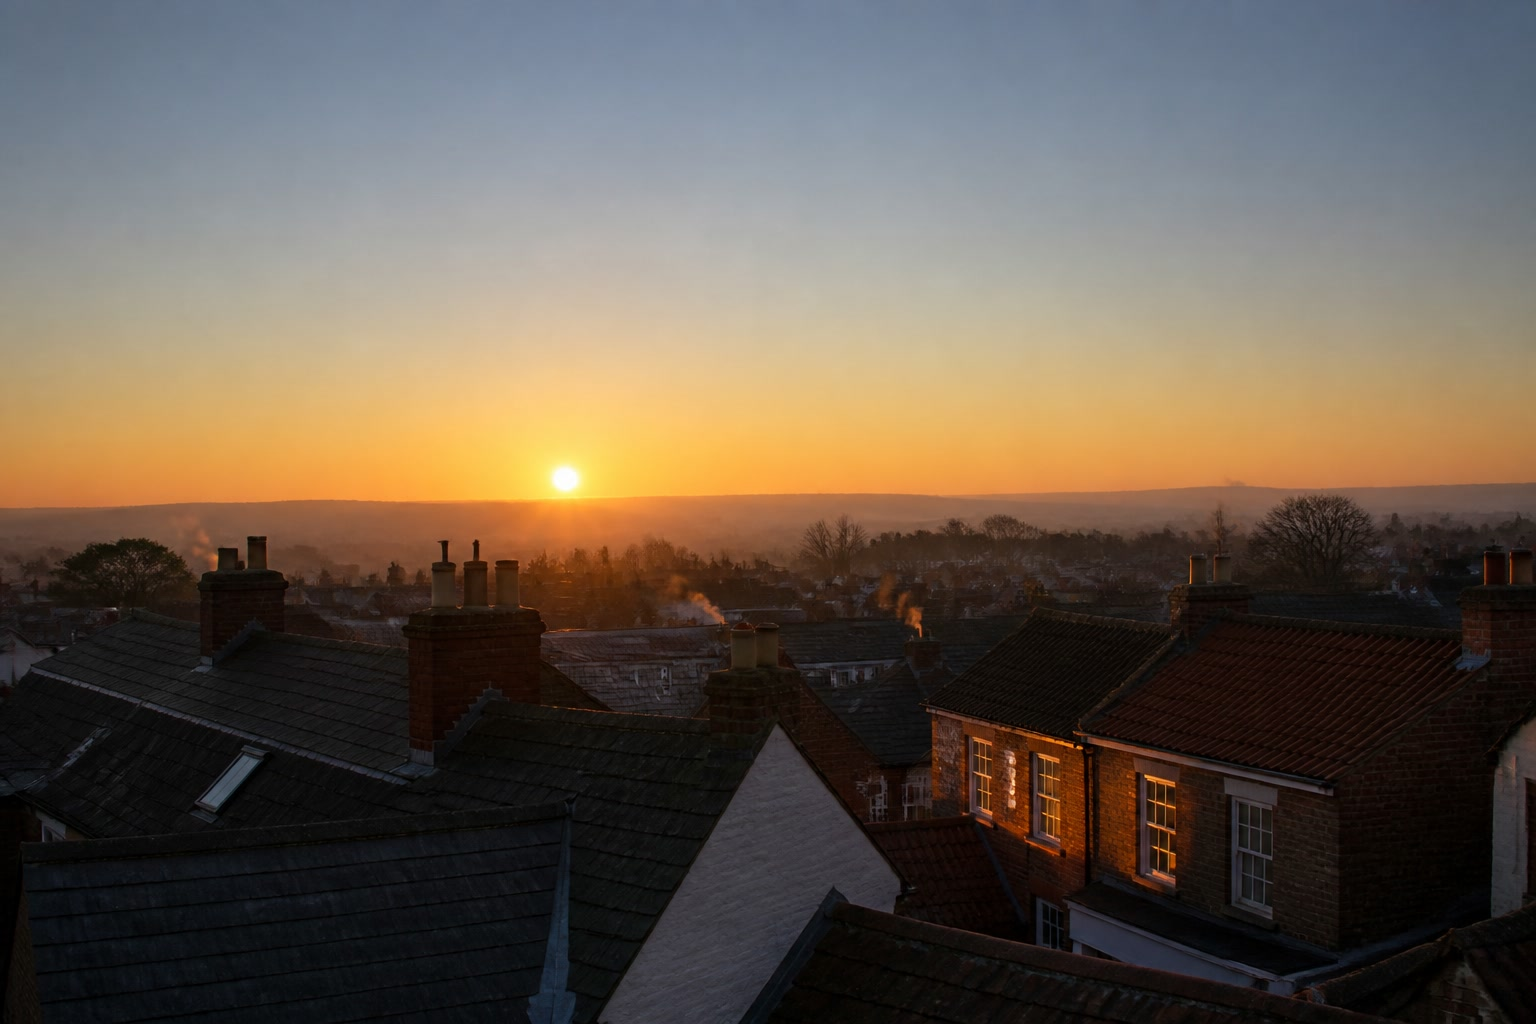
\includegraphics[width=0.6\linewidth]{images/book1/ai/g1-day-night-sunrise.jpg}

{\small 日出：太阳在屋顶上方出现，白天开始了。}
\end{omfigure}

\begin{definition}[白天与夜晚]\label{def:g1:day-and-night:daynight}
\emph{白天}\index{白天}是一天中太阳
高挂在天空、为我们带来光亮的时段。\emph{夜晚}\index{夜晚}是
太阳已不在天空、周围世界陷入黑暗的时段。
太阳出现的时刻称为\emph{日出}\index{日出}；
太阳消失的时刻称为\emph{日落}\index{日落}。
\end{definition}

\begin{remark}[白天的大光源]\label{rem:g1:day-and-night:lamp}
回想上一章的光源：白天，太阳就是
同时照亮整个世界的光源 --- 每条街道、
每个操场、每片海洋。夜里我们只能用小光源：
灯、手电筒，还有星星。这就是为什么即使灯亮着，夜晚依然很暗，
因为再小的灯也无法替代那个大光源。
\end{remark}

\begin{example}[节律在重复]\label{ex:g1:day-and-night:rhythm}
早晨、正午、傍晚、夜晚 --- 然后又是早晨。
这节律从未中断过：每个夜晚之后是白天，
每个白天之后是夜晚。这个轮子转一整圈，即一个白天\emph{加上}
一个夜晚，正是日历所计的：星期一、星期二、
星期三，每一天都是轮子转过的一圈。
\end{example}

\section{太阳夜里去了哪里？}

夜里，太阳依然在照耀 --- 只是不照在我们身上。我们睡觉时，它的
光照在地球另一侧的孩子身上，那里正是
他们的正午。太阳并没有熄灭，是
\emph{我们}转过身，背对了它。

\begin{example}[旋转的地球]\label{ex:g1:day-and-night:spinning}
地球 --- 我们都生活其上的巨大球体 --- 像旋转木马一样缓缓自转，
我们也随之转动。当球面上我们所在的一侧面向
太阳时，我们便有了白天。地球继续转动，我们这一侧
逐渐远离阳光，滑入黑暗：先是傍晚，然后是夜晚。继续转动，
我们这一侧又转回光亮之中：日出！太阳
只是\emph{看起来}横穿过我们的天空 --- 真正在移动的是
脚下的大地。
\end{example}

\begin{omfigure}
\begin{tikzpicture}[scale=0.85]
  \fill[omThm] (0.8,2.0) circle (0.5);
  \foreach \a in {0,30,...,330} {
    \draw[omThm] (0.8,2.0) ++(\a:0.7) -- ++(\a:0.3);
  }
  \node[below, font=\small] at (0.8,1.2) {太阳};
  \draw[thick] (7.0,2.0) circle (1.5);
  \begin{scope}
    \clip (7.0,2.0) circle (1.5);
    \fill[omExo, opacity=0.4] (7.0,0.4) rectangle (8.9,3.6);
  \end{scope}
  % the tilted spin axis, poking out of both poles
  \draw[thick, dash pattern=on 3pt off 2pt] (6.26,0.30) -- (7.74,3.70);
  % rotation arrow circling the axis near the north pole
  \begin{scope}[shift={(7.65,3.49)}, rotate=-23.5]
    \draw[-Stealth, thick, omDef]
      (-0.799,-0.082) arc (200:345:0.85 and 0.24);
  \end{scope}
  \fill[omDef] (5.62,2.5) circle (0.1);
  \node[left, font=\small] at (5.5,2.6) {此处是白天};
  \fill[omDef] (8.38,2.5) circle (0.1);
  \node[right, font=\small] at (8.5,2.6) {此处是夜晚};
  \node[font=\small, align=center] at (10.6,3.75)
    {地球绕倾斜的\\地轴自转};
  \draw[omExo, very thin] (9.5,3.6) -- (8.55,3.3);
\end{tikzpicture}

{\small 阳光下的地球：面向太阳的一侧
处于白天，背向太阳的一侧处于夜晚。缓慢的自转使二者轮换。}
\end{omfigure}

\begin{method}[试一试：做地球]\label{met:g1:day-and-night:beearth}
需要在暗室里准备一盏灯，还需要你自己。
\begin{enumerate}
  \item 灯代表太阳；你的头代表地球；你的鼻子代表
        你所在的城镇。
  \item 面向灯：灯光照在你的脸上 --- 你所在的城镇处于白天。
  \item 原地慢慢转身。光线从你的脸颊滑过：
        这时是傍晚。
  \item 后脑勺朝向灯：你的脸处于黑暗中 ---
        你所在的城镇是夜晚。
  \item 继续转身，直到光线重新照到你的脸颊：日出！
\end{enumerate}
你转一整圈，你的鼻子就经历了一个完整的昼夜。
\end{method}

\begin{remark}[太阳从不关闭]\label{rem:g1:day-and-night:neveroff}
在\cref{met:g1:day-and-night:beearth}的游戏中，灯
一直亮着 --- 只是你的转动使明与暗在你的脸上轮流出现。
真实的太阳也是如此：它
整夜都在发光，只是照在地球的另一侧。夜晚并非太阳
在休息，而是我们所在的这一侧球面背向了它。
\end{remark}

\section{练习}

\begin{exercise}[$\star$]\label{exo:g1:day-and-night:1}
从早晨开始排列：中午；\ 日出；\ 夜晚；
\ 日落；\ 下午。
\end{exercise}

\begin{exercise}[$\star$]\label{exo:g1:day-and-night:2}
中午时太阳在哪里：是靠近屋顶的低处，还是
最高点？那一时刻你的影子是长还是短？（想一想
上一章。）
\end{exercise}

\begin{exercise}[$\star$]\label{exo:g1:day-and-night:3}
太阳每天早晨是否都从你家的同一侧升起，还是
每天从不同的一侧升起？今天怎样才能验证明天的情况？
\end{exercise}

\begin{exercise}[$\star$]\label{exo:g1:day-and-night:4}
判断对错：“夜晚时太阳会关闭。”请用
\cref{rem:g1:day-and-night:neveroff}解释你的答案。
\end{exercise}

\begin{exercise}[$\star$]\label{exo:g1:day-and-night:5}
你在早晨的光线中吃早餐时，
地球另一侧的孩子此时最可能在做什么？
\end{exercise}

\begin{exercise}[$\star$]\label{exo:g1:day-and-night:6}
用一盏灯玩\cref{met:g1:day-and-night:beearth}。当光线
照在你的右脸颊上，并且你沿同一方向继续转动时，
你的鼻子接下来会迎来什么：日出还是日落？
\end{exercise}

\begin{exercise}[$\star$]\label{exo:g1:day-and-night:7}
哪一个才是真正的“旅行者”：划过天空的太阳，还是
脚下的大地？请用自己的话说一说。
\end{exercise}

\begin{exercise}[$\star$]\label{exo:g1:day-and-night:8}
用日历数一数：一周里有几次日出？
有几个夜晚？
\end{exercise}

\begin{exercise}[$\star\star$]\label{exo:g1:day-and-night:9}
佐伊说：“如果地球停止自转，我们的城镇将永远是白天
。”她说得对吗？地球另一侧的孩子会对她的
想法怎么看？
\end{exercise}
